\begin{frame}[fragile]{On the Agenda}

\begin{itemize}
\tightlist
\item
  Effective Groups (Inspired by
  \href{https://cs.illinois.edu/directory/profile/bpbailey}{Prof.~Brian
  Bailey})

  \begin{itemize}
  \tightlist
  \item
    Why groups?
  \item
    Stages of Group Development
  \item
    Group Norms
  \end{itemize}
\item
  Control Structures

  \begin{itemize}
  \tightlist
  \item
    \texttt{if/else}, \texttt{if/elseif/else}, \texttt{switch}
  \item
    Ternary Operator
  \item
    While
  \item
    Do-While
  \item
    For
  \end{itemize}
\item
  Big O

  \begin{itemize}
  \tightlist
  \item
    Notation
  \item
    Examples
  \item
    Drawbacks
  \end{itemize}
\end{itemize}

\end{frame}

\begin{frame}{Grouping Brainstorming}

Form a group of 2-3 people around you.

Take three minutes to answer the following:

\begin{itemize}
\tightlist
\item
  What was your \emph{best} group experience?
\item
  What do you like the most about group work?
\item
  What techniques worked well for groups?
\end{itemize}

Take (another) three minutes to answer the following:

\begin{itemize}
\tightlist
\item
  What was your \emph{wurst} group experience?
\item
  What do you \emph{dislike} the most about group work?
\end{itemize}

\end{frame}

\begin{frame}{Did you introduce yourself?}

\begin{itemize}
\tightlist
\item
  When you started to talk with those around you, did you
  \textbf{introduce} yourself first?
\item
  Or did you just jump into the task?
\item
  \textbf{Always introduce yourself \emph{before} starting the task!}
\end{itemize}

\end{frame}

\begin{frame}{Why Group?}

\begin{itemize}
\tightlist
\item
  Exposure to \emph{new} viewpoints from different fields and life
  experiences
\item
  Improves creativity and overall work quality (4 eyes vs.~2 eyes)
\item
  Constructive dialog and increased internal group motivation
\item
  Personal accountability to the team
\item
  Friendship
\item
  Prepares you for a team-environment in the workplace or a research
  group.
\end{itemize}

\end{frame}

\begin{frame}{Statistics \textbf{is} a group effort}

\begin{figure}[htbp]
\centering
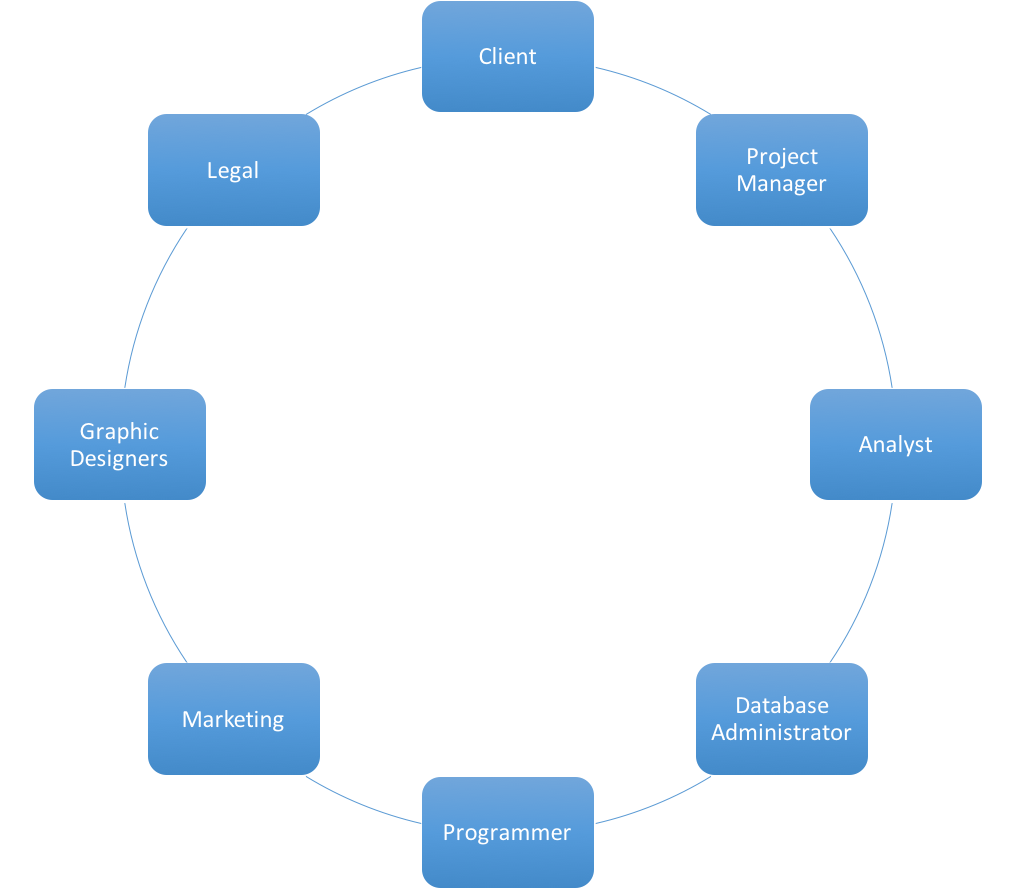
\includegraphics{figures/circle_of_statistics.png}
\caption{Process of an Analysis}
\end{figure}

\end{frame}

\begin{frame}{Stages of Group Development (Tuckman and Jensen 2010)}

\begin{figure}[htbp]
\centering
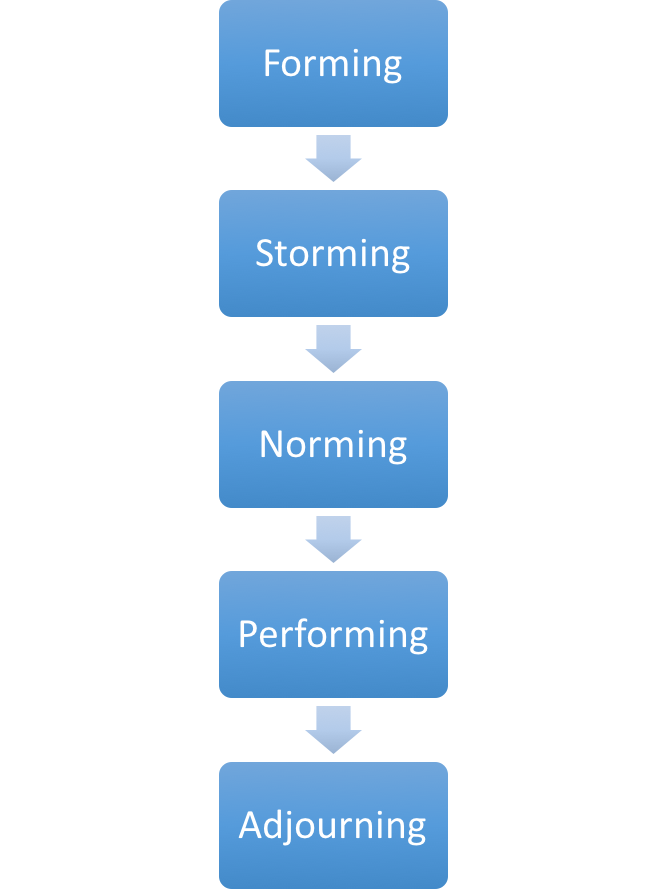
\includegraphics{figures/stages_of_group_development.png}
\caption{Small Group Development}
\end{figure}

\end{frame}

\begin{frame}{Forming (Honeymoon Stage)}

\begin{itemize}
\tightlist
\item
  \textbf{Excitement}

  \begin{itemize}
  \tightlist
  \item
    New experiences and people
  \end{itemize}
\item
  \textbf{Eagerness}

  \begin{itemize}
  \tightlist
  \item
    Working on a common new task
  \end{itemize}
\item
  \textbf{High Expectations}

  \begin{itemize}
  \tightlist
  \item
    We will be able to get a good grade.
  \item
    We can use \emph{this}
  \end{itemize}
\item
  \textbf{Anxiety}

  \begin{itemize}
  \tightlist
  \item
    Will I fit in?
  \item
    Am I able to contribute?
  \end{itemize}
\end{itemize}

\end{frame}

\begin{frame}{Forming (Honeymoon Stage)}

Combat the \textbf{anxiety} with an ice-breaker activity:

\begin{itemize}
\tightlist
\item
  Try to come up with a team name
\item
  Talk about the weather
\item
  Fact or Fiction

  \begin{itemize}
  \tightlist
  \item
    Write 2 facts and 1 fictional item
  \item
    The group guesses the fictional item.
  \end{itemize}
\end{itemize}

\end{frame}

\begin{frame}{Storming (Internal Strife)}

\begin{itemize}
\tightlist
\item
  As you begin to work, group structure will form to ensure goals are
  met

  \begin{itemize}
  \tightlist
  \item
    Who is the leader? Who can write well? Who is able to program? And
    so on\ldots{}
  \end{itemize}
\item
  Watch out for \textbf{conflict} due to group structure disagreements
  on roles and processes.

  \begin{itemize}
  \tightlist
  \item
    Form a consensus on different roles and processes.
  \end{itemize}
\item
  Some groups may skip this stage and jump to \textbf{norming}.
\end{itemize}

\end{frame}

\begin{frame}{Norming (Resolution)}

\begin{itemize}
\tightlist
\item
  Conflicts in \textbf{Storming} are resolved due to a formed consensus.

  \begin{itemize}
  \tightlist
  \item
    Team member idiosyncrasy are accepted or corrected.
  \end{itemize}
\item
  Team members begins focusing on the goal as group members take on
  their responsibilities.
\item
  Overall, the team is ready to collaborate together toward a common
  goal.

  \begin{itemize}
  \tightlist
  \item
    Watch out for suppressing conflict by avoiding discussing
    controversial ideas!
  \end{itemize}
\end{itemize}

\end{frame}

\begin{frame}{Performing (Working)}

\begin{itemize}
\tightlist
\item
  Team members work fluidly together to finish the common goals.
\item
  Main stage of the group process
\item
  Teams may stumble back to prior stages or never reach this stage.
\end{itemize}

\end{frame}

\begin{frame}{Adjourning / Mourning (Finale)}

\begin{itemize}
\tightlist
\item
  Completion of the common task and the end of the group

  \begin{itemize}
  \tightlist
  \item
    Anxiousness, Sadness, or Relief
  \end{itemize}
\item
  Reflect on how the group worked and channel it into the next group
\item
  Congratulate team members on a job well down and note the individual
  contributions
\item
  Finish any other administrative tasks

  \begin{itemize}
  \tightlist
  \item
    e.g.~Write a peer review of each group member.
  \end{itemize}
\end{itemize}

\end{frame}

\begin{frame}{Tips for Group Work - Part 1}

\begin{itemize}
\tightlist
\item
  \textbf{Work Hard}

  \begin{itemize}
  \tightlist
  \item
    Do your share and more to set both an example and communicate
    willingness
  \end{itemize}
\item
  \textbf{Include All Team Members in Group Activities}

  \begin{itemize}
  \tightlist
  \item
    Being left out \emph{stinks} and its hard to get over.
  \item
    Try to provide reasonable deadlines for time sensitive decisions.
  \end{itemize}
\item
  \textbf{Take Turns}

  \begin{itemize}
  \tightlist
  \item
    Cycle leadership, following, organization, note taker, and
    discussant roles.
  \item
    Promotes an atmosphere of shared equity.
  \end{itemize}
\end{itemize}

\end{frame}

\begin{frame}{Tips for Group Work - Part 2}

\begin{itemize}
\tightlist
\item
  \textbf{Constructive Dialog}

  \begin{itemize}
  \tightlist
  \item
    Focus on the \textbf{idea} and \textbf{not} the person proposing it.
  \item
    Try to \textbf{extend}, \textbf{shape}, or \textbf{add} to a
    proposed idea
  \end{itemize}
\item
  \textbf{Data Driven Decisions}

  \begin{itemize}
  \tightlist
  \item
    Avoid ``I don't like it'' in favor of evidence.
  \item
    Personal preferences are not evidence and are hard to articulate.
  \end{itemize}
\item
  \textbf{Focus on the Task}

  \begin{itemize}
  \tightlist
  \item
    Utilize your time appropriately by being prepared and ontime.
  \end{itemize}
\end{itemize}

\end{frame}

\begin{frame}{Tips for Group Work - Part 3}

\begin{itemize}
\tightlist
\item
  \textbf{A Happy Group Makes for Happy Group Members}

  \begin{itemize}
  \tightlist
  \item
    Make a positive statement in the beginning
  \item
    Bring something to the meeting (e.g.~food, drinks, et cetera)
  \end{itemize}
\item
  \textbf{Move On}

  \begin{itemize}
  \tightlist
  \item
    Don't sweat not being able to agree
  \item
    Take breaks and revisit the idea later.
  \end{itemize}
\item
  \textbf{Avoid Assigning Blame}

  \begin{itemize}
  \tightlist
  \item
    Suggest ideas to fix problems
  \item
    Try to understand the other persons viewpoint
  \end{itemize}
\item
  \textbf{Deliverables}

  \begin{itemize}
  \tightlist
  \item
    Figure out \textbf{who} is doing \textbf{what} task and
    \textbf{when} it will be done.
  \end{itemize}
\end{itemize}

\end{frame}

\begin{frame}{Tools for Collaboration}

\begin{itemize}
\tightlist
\item
  \textbf{Create a shared space to store all your materials}

  \begin{itemize}
  \tightlist
  \item
    \href{https://wiki.cites.illinois.edu/wiki/}{CITES Wiki}
  \item
    \href{www.dropbox.com}{Dropbox} (2.5 gigs),
    \href{https://app.box.com/}{BoxSync} (50 gigs), \&
    \href{https://drive.google.com}{Google Drive} (Unlimited Storage!!!)
  \end{itemize}
\item
  \textbf{Group Document Editing}

  \begin{itemize}
  \tightlist
  \item
    \href{https://docs.google.com}{Google Docs}
  \item
    \href{www.sharelatex.com}{ShareLaTeX} (1 Collaborator + Supports
    Knitr)
  \item
    \href{https://www.overleaf.com/}{Overleaf} (1 gig + unlimited
    collaborators)
  \item
    MS Word's
    \href{https://support.office.com/en-us/article/Track-changes-while-you-edit-024158a3-7e62-4f05-8bb7-dc3ecf0295c4}{Track
    Document Changes}
  \end{itemize}
\item
  \textbf{Use a discussion board}

  \begin{itemize}
  \tightlist
  \item
    \href{https://groups.google.com/forum/\#!overview}{Google Groups}
  \item
    \href{http://www.cites.illinois.edu/maillist/}{Illinois Mailing
    Lists}
  \end{itemize}
\item
  \textbf{Use a Versioning Tool}

  \begin{itemize}
  \tightlist
  \item
    \href{http://git-scm.com/downloads}{git}
  \item
    \href{https://subversion.apache.org/packages.html}{svn}
  \end{itemize}
\item
  \textbf{Remote Communications Tools}

  \begin{itemize}
  \tightlist
  \item
    \href{http://www.skype.com/en/download-skype/skype-for-computer/}{Skype}
  \item
    \href{https://www.google.com/hangouts}{Google Hangouts}
  \end{itemize}
\end{itemize}

\end{frame}

\begin{frame}{One Last Secret}

\textbf{Groups that do well tend to sit together in class.}

\begin{center}
\includegraphics[width=150px]{figures/smiley_face} \end{center}

\end{frame}

\begin{frame}{Summary of Group Work}

\begin{itemize}
\tightlist
\item
  In the industry and academia, working in groups is the standard.

  \begin{itemize}
  \tightlist
  \item
    \textbf{Avoid being a lone wolf}
  \end{itemize}
\item
  Provided tips and tricks to working in a group
\item
  Emphasized \textbf{tool} usage.
\end{itemize}

\end{frame}

\begin{frame}{Coming up next\ldots{}}

Next on the agenda is talking about \textbf{Control Structures} in
\emph{R}.

\end{frame}

\begin{frame}{Control Structures and Flow of Control}

\begin{itemize}
\item
  A \textbf{control structure} is a piece of code whose \textbf{analysis
  of a variable} results in a \textbf{choice being made as to the
  direction} the program should go.
\item
  Meanwhile, the \textbf{Flow of Control} specifies the
  \textbf{direction} the program takes or \textbf{flows} when given
  conditions and parameters.
\end{itemize}

\end{frame}

\begin{frame}{Types of Control Structures:}

There are \textbf{three} different types of control structures.

\begin{itemize}
\tightlist
\item
  \textbf{Sequential:} Executes code statements one line after another

  \begin{itemize}
  \tightlist
  \item
    Exactly adhering to an algorithm like creating a cake from a recipe.
  \end{itemize}
\item
  \textbf{Selection:} Allows for decisions between 2 or more alternative
  paths.

  \begin{itemize}
  \tightlist
  \item
    Making a choice as to whether I want a
    \href{http://lp.starbucks.com/coldbrew}{Cold Brew} or
    \href{http://www.starbucks.com/menu/drinks/iced-coffee/iced-coffee}{Iced
    Coffee} from \emph{Starbucks}.
  \end{itemize}
\item
  \textbf{Iteration:} Enables the looping or repeating of a section code
  multiple times.

  \begin{itemize}
  \tightlist
  \item
    Saying the same words
    \href{https://www.youtube.com/watch?v=NP0mQeLWCCo}{over and over
    again}.
  \end{itemize}
\end{itemize}

\end{frame}

\begin{frame}[fragile]{Logical Operators}

To control the structure, we sometimes must make \textbf{decisions} that
have different cases based on a \emph{boolean} (0 or 1) expression.

A few such structures are given as:

\begin{longtable}[c]{@{}ll@{}}
\toprule
Operator & Explanation\tabularnewline
\midrule
\endhead
\texttt{x\ ==\ y} & \texttt{x} equal to \texttt{y}\tabularnewline
\texttt{x\ !=\ y} & \texttt{x} not equal to \texttt{y}\tabularnewline
\texttt{x\ \textless{}\ y} & \texttt{x} less than
\texttt{y}\tabularnewline
\texttt{x\ \textgreater{}\ y} & \texttt{x} greater than
\texttt{y}\tabularnewline
\texttt{x\ \textless{}=\ y} & \texttt{x} less than or equal to
\texttt{y}\tabularnewline
\texttt{x\ \textgreater{}=\ y} & \texttt{x} greater than or equal to
\texttt{y}\tabularnewline
\bottomrule
\end{longtable}

\end{frame}

\begin{frame}[fragile]{Combining Logical Operators}

We can combine logical operators using:

\begin{longtable}[c]{@{}ll@{}}
\toprule
Operator & Explanation\tabularnewline
\midrule
\endhead
\texttt{!x} & not \texttt{x}\tabularnewline
\texttt{x\ \textbar{}\textbar{}\ y} & \texttt{x} or
\texttt{y}\tabularnewline
\texttt{x\ \&\&\ y} & \texttt{x} and \texttt{y}\tabularnewline
\bottomrule
\end{longtable}

\end{frame}

\begin{frame}[fragile]{Examples of Logical Operators}

\begin{longtable}[c]{@{}lll@{}}
\toprule
Explanation & Example & Result\tabularnewline
\midrule
\endhead
\texttt{x} equal to \texttt{y} & \texttt{1\ ==\ 10} &
\texttt{FALSE}\tabularnewline
\texttt{x} not equal to \texttt{y} & \texttt{1\ !=\ 10} &
\texttt{TRUE}\tabularnewline
\texttt{x} less than \texttt{y} & \texttt{1\ \textless{}\ 10} &
\texttt{TRUE}\tabularnewline
\texttt{x} greater than \texttt{y} & \texttt{1\ \textgreater{}\ 10} &
\texttt{FALSE}\tabularnewline
\texttt{x} less than or equal to \texttt{y} &
\texttt{1\ \textless{}=\ 10} & \texttt{TRUE}\tabularnewline
\texttt{x} greater than or equal to \texttt{y} &
\texttt{1\ \textgreater{}=\ 10} & \texttt{FALSE}\tabularnewline
not \texttt{x} & \texttt{!(1\ \textless{}\ 10)} &
\texttt{FALSE}\tabularnewline
\texttt{x} or \texttt{y} & \texttt{FALSE\ \textbar{}\textbar{}\ TRUE} &
\texttt{TRUE}\tabularnewline
\texttt{x} and \texttt{y} &
\texttt{(1\ \textless{}\ 10)\ \&\&\ (15\ \textgreater{}\ 10)} &
\texttt{TRUE}\tabularnewline
\bottomrule
\end{longtable}

\end{frame}

\begin{frame}{Venn Diagrams of Logic}

\begin{center}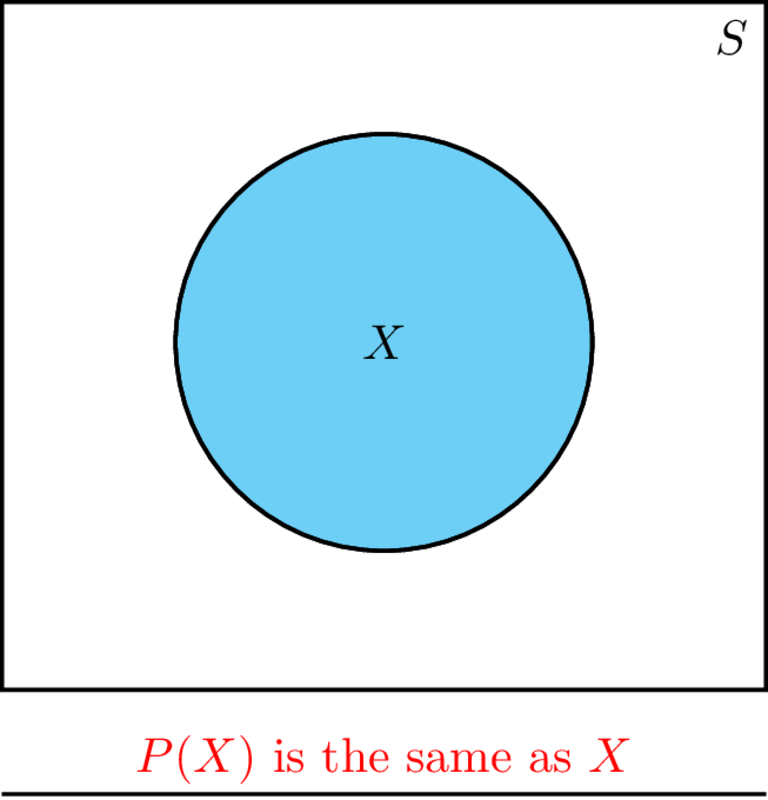
\includegraphics[width=100px]{figures/venn_diagram_x_v2} \end{center}

\begin{center}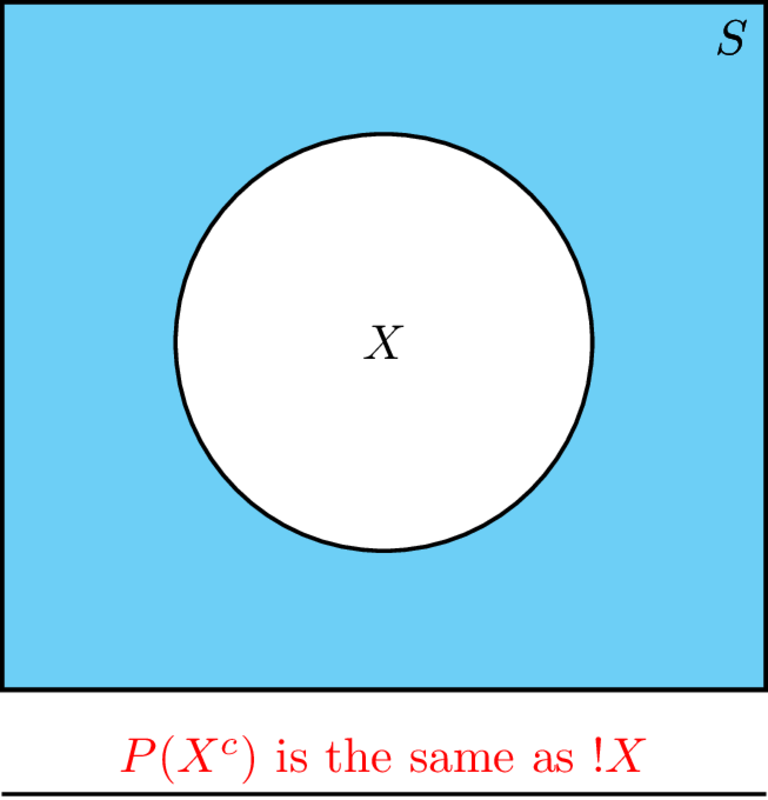
\includegraphics[width=100px]{figures/venn_diagram_notx_v2} \end{center}

\end{frame}

\begin{frame}{Venn Diagrams of Logic}

\begin{center}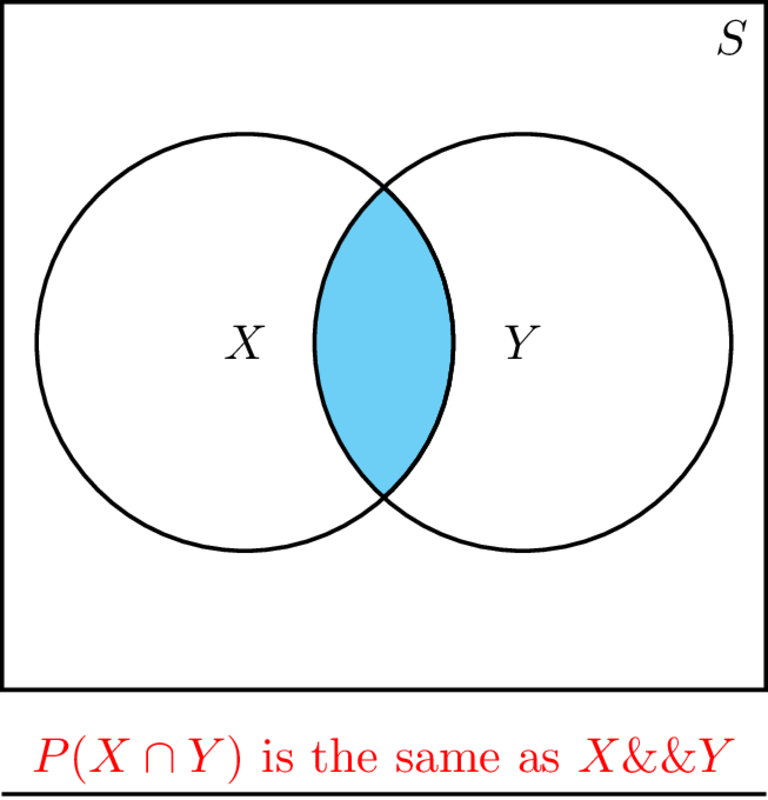
\includegraphics[width=100px]{figures/venn_diagram_xandy} \end{center}

\begin{center}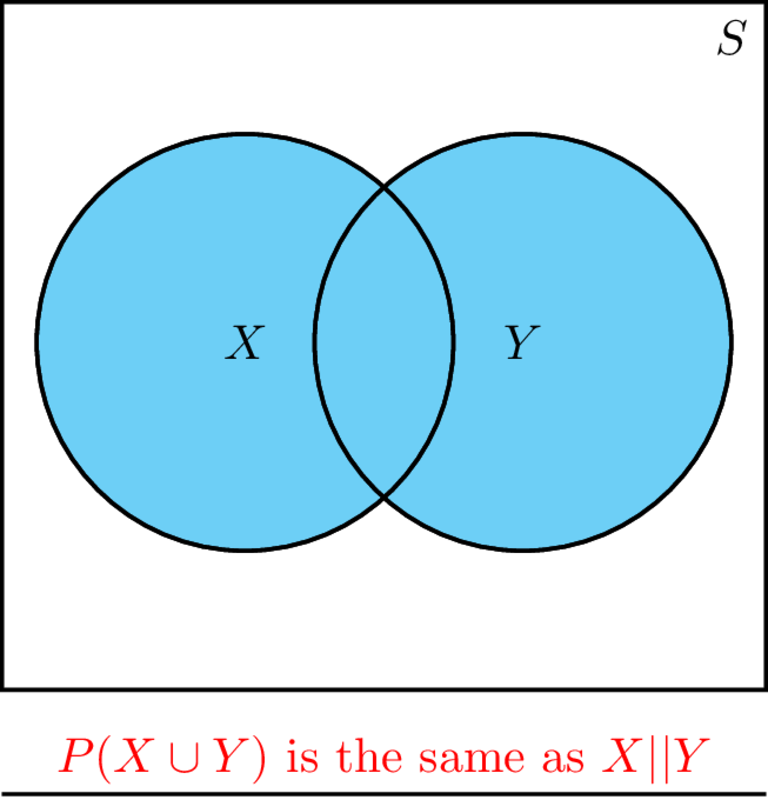
\includegraphics[width=100px]{figures/venn_diagram_xory} \end{center}

\end{frame}

\begin{frame}[fragile]{Short Circuit Evaluation}

\begin{itemize}
\tightlist
\item
  The \texttt{\&\&} and \texttt{\textbar{}\textbar{}} operators both
  have a feature called \textbf{short-circuit evaluation}.
\item
  Consider the \texttt{\&\&} (\texttt{AND}) expression
  (\texttt{x\ \&\&\ y}) \ldots{}

  \begin{itemize}
  \tightlist
  \item
    If \texttt{x} is \texttt{FALSE}, then there is no reason to evaluate
    \texttt{y} so the evaluation stops.
  \item
    Take for example a division check for zero:
  \end{itemize}
\end{itemize}

\begin{Shaded}
\begin{Highlighting}[]
\NormalTok{x =}\StringTok{ }\DecValTok{0}\NormalTok{; y =}\StringTok{ }\DecValTok{4}         \CommentTok{# Define Variables}
\NormalTok{(x !=}\StringTok{ }\DecValTok{0} \NormalTok{&&}\StringTok{  }\NormalTok{y/x >}\StringTok{ }\DecValTok{0}\NormalTok{) }\CommentTok{# Evaluates only x != 0}
                     \CommentTok{# so y/x never runs.}
\end{Highlighting}
\end{Shaded}

\begin{itemize}
\tightlist
\item
  Similarly, the \texttt{\textbar{}\textbar{}} (\texttt{OR}) expression
  (\texttt{x\ \textbar{}\textbar{}\ y}) \ldots{}

  \begin{itemize}
  \tightlist
  \item
    If \texttt{x} is \texttt{TRUE}, then whole expression is
    \texttt{TRUE} so there is no need to evaluate \texttt{y}.
  \item
    Only in the case when \texttt{x} is \texttt{FALSE} does \texttt{y}
    get evaluated.
  \end{itemize}
\end{itemize}

\end{frame}

\begin{frame}{Sequential Control}

Sequential control is the default operating behavior of a computer
program. The program will read each line one after another and execute
it.

\begin{center}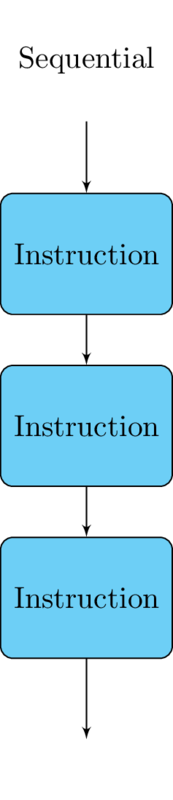
\includegraphics[width=100px]{figures/sequential_diagram} \end{center}

\end{frame}

\begin{frame}[fragile]{Selection Control}

\begin{itemize}
\tightlist
\item
  \textbf{Selection:} Allows for decisions between 2 or more alternative
  paths.

  \begin{itemize}
  \tightlist
  \item
    \texttt{if}
  \item
    \texttt{if/else}
  \item
    \texttt{if/elseif/else}
  \item
    \texttt{switch}
  \end{itemize}
\end{itemize}

\begin{center}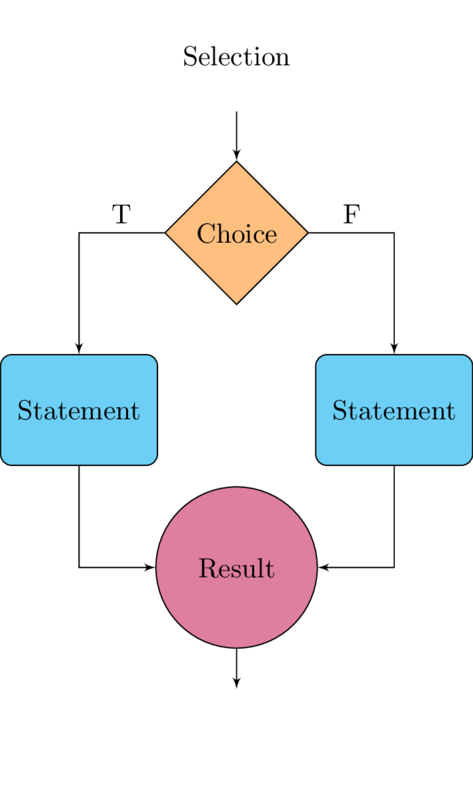
\includegraphics[width=100px]{figures/selection_diagram} \end{center}

\end{frame}

\begin{frame}[fragile]{Selection Control - \texttt{if} and
\texttt{if/else}}

The \texttt{if} statement provides the ability to execute code only when
the \texttt{expression} is \texttt{TRUE} like so:

\begin{Shaded}
\begin{Highlighting}[]
\NormalTok{if (expression)\{ }\CommentTok{# True Case}
  \CommentTok{# statement}
\NormalTok{\}}
\end{Highlighting}
\end{Shaded}

Traditionally, one would normally use \texttt{if/else} statement to
address both \texttt{TRUE} and \texttt{FALSE} cases:

\begin{Shaded}
\begin{Highlighting}[]
\NormalTok{if (expression)\{ }\CommentTok{# True Case}
  \CommentTok{# statement}
\NormalTok{\} else \{         }\CommentTok{# False Case}
  \CommentTok{# statement}
\NormalTok{\}}
\end{Highlighting}
\end{Shaded}

\end{frame}

\begin{frame}[fragile]{Selection Control - \texttt{if} and
\texttt{if/else} Examples}

Selection control in action:

\begin{Shaded}
\begin{Highlighting}[]
\NormalTok{x =}\StringTok{ }\DecValTok{2}
\NormalTok{if (x >}\StringTok{ }\DecValTok{0}\NormalTok{)\{   }\CommentTok{# Detect if x is a positive number}
  \KeywordTok{cat}\NormalTok{(x,}\StringTok{"}\CharTok{\textbackslash{}n}\StringTok{"}\NormalTok{) }\CommentTok{# Print `x` to console }
\NormalTok{\}}
\end{Highlighting}
\end{Shaded}

\begin{verbatim}
## 2
\end{verbatim}

\begin{Shaded}
\begin{Highlighting}[]
\NormalTok{if (x !=}\StringTok{ }\DecValTok{42}\NormalTok{)\{    }\CommentTok{# True Case}
  \KeywordTok{cat}\NormalTok{(}\StringTok{"This is not the meaning of life}\CharTok{\textbackslash{}n}\StringTok{"}\NormalTok{) }
  \NormalTok{x =}\StringTok{ }\DecValTok{42}
\NormalTok{\} else \{         }\CommentTok{# False Case}
  \KeywordTok{cat}\NormalTok{(}\StringTok{"This is the meaning of life!}\CharTok{\textbackslash{}n}\StringTok{"}\NormalTok{) }
\NormalTok{\}}
\end{Highlighting}
\end{Shaded}

\begin{verbatim}
## This is not the meaning of life
\end{verbatim}

\end{frame}

\begin{frame}[fragile]{Selection Control - \texttt{if} and
\texttt{if/else} Example}

Consider the following \texttt{if/else} statement, how will the program
operator?

\begin{Shaded}
\begin{Highlighting}[]
\NormalTok{if (x <}\StringTok{ }\DecValTok{1}\NormalTok{)}
  \KeywordTok{cat}\NormalTok{(}\StringTok{"True}\CharTok{\textbackslash{}n}\StringTok{"}\NormalTok{)}
\NormalTok{else}
  \KeywordTok{cat}\NormalTok{(}\StringTok{"False}\CharTok{\textbackslash{}n}\StringTok{"}\NormalTok{)}
  \KeywordTok{cat}\NormalTok{(}\StringTok{"Too bad!}\CharTok{\textbackslash{}n}\StringTok{"}\NormalTok{);}
\end{Highlighting}
\end{Shaded}

\end{frame}

\begin{frame}[fragile]{Selection Control - \texttt{if} and
\texttt{if/else} Common Mistakes}

A few other problematic areas when working with \texttt{expressions} for
\texttt{if} statements in R:

\textbf{Example 1:}

\begin{Shaded}
\begin{Highlighting}[]
\NormalTok{user_input =}\StringTok{ }\KeywordTok{readline}\NormalTok{(}\DataTypeTok{prompt=}\StringTok{"Enter y or n:"}\NormalTok{)}
\NormalTok{if (user_input !=}\StringTok{ "y"} \NormalTok{||}\StringTok{ }\NormalTok{user_input !=}\StringTok{ "n"}\NormalTok{)}
  \KeywordTok{cat}\NormalTok{(}\StringTok{"Please enter either y or n (y for yes and n for no)}\CharTok{\textbackslash{}n}\StringTok{"}\NormalTok{)}
\end{Highlighting}
\end{Shaded}

\textbf{Example 2:}

\begin{Shaded}
\begin{Highlighting}[]
\NormalTok{x =}\StringTok{ }\DecValTok{9}\NormalTok{; y =}\StringTok{ }\DecValTok{20}
\NormalTok{if (x <}\StringTok{ }\DecValTok{10}\NormalTok{) &&}\StringTok{ }\NormalTok{(y <}\StringTok{ }\DecValTok{35}\NormalTok{)}
  \KeywordTok{cat}\NormalTok{(}\StringTok{"Bingo was his name!}\CharTok{\textbackslash{}n}\StringTok{"}\NormalTok{)}
\end{Highlighting}
\end{Shaded}

\textbf{Example 3:}

\begin{Shaded}
\begin{Highlighting}[]
\NormalTok{x =}\StringTok{ }\DecValTok{43}
\NormalTok{if (x ==}\StringTok{ }\DecValTok{42} \NormalTok{||}\StringTok{ }\DecValTok{43} \NormalTok{||}\StringTok{ }\DecValTok{44}\NormalTok{)}
  \KeywordTok{cat}\NormalTok{(}\StringTok{"That's close to my age!}\CharTok{\textbackslash{}n}\StringTok{"}\NormalTok{)}
\end{Highlighting}
\end{Shaded}

\end{frame}

\begin{frame}[fragile]{Selection Control - \texttt{if} and
\texttt{if/else} Common Mistakes}

\textbf{Example 4:}

\begin{Shaded}
\begin{Highlighting}[]
\NormalTok{x =}\StringTok{ }\KeywordTok{seq}\NormalTok{(}\DecValTok{0}\NormalTok{,}\DecValTok{1}\NormalTok{,}\DataTypeTok{by =} \FloatTok{0.1}\NormalTok{)}
\NormalTok{y =}\StringTok{ }\KeywordTok{seq}\NormalTok{(.}\DecValTok{1}\NormalTok{,}\FloatTok{1.1}\NormalTok{,}\DataTypeTok{by =} \FloatTok{0.1}\NormalTok{)}
\NormalTok{if (x <}\StringTok{ }\NormalTok{y)}
  \OtherTok{TRUE}
\end{Highlighting}
\end{Shaded}

\end{frame}

\begin{frame}[fragile]{Selection Control - Vectorized \texttt{if/else}}

In the case of the last \texttt{if} statement, we have the ability to
use \emph{R}'s vectorized \texttt{ifelse()}

\begin{Shaded}
\begin{Highlighting}[]
\KeywordTok{ifelse}\NormalTok{(expression, }\OtherTok{TRUE}\NormalTok{-CONDITION, }\OtherTok{FALSE}\NormalTok{-CONDITION)}
\end{Highlighting}
\end{Shaded}

Example:

\begin{Shaded}
\begin{Highlighting}[]
\NormalTok{x =}\StringTok{ }\KeywordTok{seq}\NormalTok{(}\DecValTok{0}\NormalTok{,}\DecValTok{1}\NormalTok{,}\DataTypeTok{by =} \FloatTok{0.1}\NormalTok{)}
\NormalTok{y =}\StringTok{ }\KeywordTok{seq}\NormalTok{(}\FloatTok{0.1}\NormalTok{,}\FloatTok{1.1}\NormalTok{,}\DataTypeTok{by =} \FloatTok{0.1}\NormalTok{)}
\KeywordTok{ifelse}\NormalTok{(x <}\StringTok{ }\NormalTok{y, }\OtherTok{TRUE}\NormalTok{, }\OtherTok{FALSE}\NormalTok{)}
\end{Highlighting}
\end{Shaded}

\begin{verbatim}
##  [1] TRUE TRUE TRUE TRUE TRUE TRUE TRUE TRUE TRUE TRUE TRUE
\end{verbatim}

\textbf{Note:} Watch out for vector recycling!

\end{frame}

\begin{frame}[fragile]{Selection Control - \texttt{if/elseif/else}}

Sometimes, we may wish to group together certain conditions

\begin{Shaded}
\begin{Highlighting}[]
\NormalTok{if(expression)\{}
    \CommentTok{# statements}
\NormalTok{\} else if (expression2)\{}
    \CommentTok{# statements}
\NormalTok{\} else \{ }
    \CommentTok{# statements}
\NormalTok{\}}
\end{Highlighting}
\end{Shaded}

In this case, the first statement is checked, if it does not contain the
correct value the next statement is check and so until either one of the
\texttt{expression}s is true or it arrives at the \texttt{else}
condition.

\end{frame}

\begin{frame}[fragile]{Selection Control - \texttt{if/elseif/else}}

\textbf{Example:}

\begin{Shaded}
\begin{Highlighting}[]
\NormalTok{x =}\StringTok{ }\DecValTok{3}
\NormalTok{if (x ==}\DecValTok{1}\NormalTok{) \{}
  \KeywordTok{cat}\NormalTok{(}\StringTok{'Equal}\CharTok{\textbackslash{}n}\StringTok{'}\NormalTok{)}
\NormalTok{\} else if (x >}\StringTok{ }\DecValTok{1}\NormalTok{)\{}
  \KeywordTok{cat}\NormalTok{(}\StringTok{'Greater Than}\CharTok{\textbackslash{}n}\StringTok{'}\NormalTok{)}
\NormalTok{\} else \{}
  \KeywordTok{cat}\NormalTok{(}\StringTok{'Less Than}\CharTok{\textbackslash{}n}\StringTok{'}\NormalTok{)}
\NormalTok{\}}
\end{Highlighting}
\end{Shaded}

\begin{verbatim}
## Greater Than
\end{verbatim}

\end{frame}

\begin{frame}[fragile]{Selection Control - \texttt{if/elseif/else}}

An equivalent, though, less desirable statement could be written using
only \texttt{if/else}

\begin{Shaded}
\begin{Highlighting}[]
\NormalTok{x =}\StringTok{ }\DecValTok{3}
\NormalTok{if (x ==}\StringTok{ }\DecValTok{42}\NormalTok{) \{}
  \KeywordTok{cat}\NormalTok{(}\StringTok{'Equal}\CharTok{\textbackslash{}n}\StringTok{'}\NormalTok{)}
\NormalTok{\} else \{}
  \NormalTok{if (x >}\StringTok{ }\DecValTok{42}\NormalTok{)\{}
    \KeywordTok{cat}\NormalTok{(}\StringTok{'Greater Than}\CharTok{\textbackslash{}n}\StringTok{'}\NormalTok{)}
  \NormalTok{\} else \{}
    \KeywordTok{cat}\NormalTok{(}\StringTok{'Less Than}\CharTok{\textbackslash{}n}\StringTok{'}\NormalTok{)}
  \NormalTok{\}}
\NormalTok{\}}
\end{Highlighting}
\end{Shaded}

\begin{verbatim}
## Less Than
\end{verbatim}

\textbf{Discussion:} Why might structuring the \texttt{if} this way be
not so ideal?

\end{frame}

\begin{frame}[fragile]{Selection Control - Vectorized
\texttt{if/elseif/else}}

Following in the previous examples footsteps, we can write a vectorized
version to process multiple observations via:

\begin{Shaded}
\begin{Highlighting}[]
\KeywordTok{ifelse}\NormalTok{(x ==}\StringTok{ }\DecValTok{42}\NormalTok{, }\StringTok{'Equal'}\NormalTok{, }
       \KeywordTok{ifelse}\NormalTok{(x >}\StringTok{ }\DecValTok{42}\NormalTok{, }\StringTok{'Greater Than'}\NormalTok{, }\StringTok{'Less Than'}\NormalTok{))}
\end{Highlighting}
\end{Shaded}

\begin{verbatim}
## [1] "Less Than"
\end{verbatim}

\end{frame}

\begin{frame}[fragile]{Selection - Ternary Operator}

Previously, we saw a \emph{vectorized} version of the ternary operator
given by \texttt{ifelse()}.

What makes a selection statement a \textbf{ternary operator} is it is
meant to be an \textbf{inline} \texttt{if/else} statement. e.g.

\begin{Shaded}
\begin{Highlighting}[]
\NormalTok{if(expression) }\OtherTok{TRUE}  \NormalTok{else  }\OtherTok{FALSE}
\end{Highlighting}
\end{Shaded}

Consider:

\begin{Shaded}
\begin{Highlighting}[]
\NormalTok{x =}\StringTok{ }\DecValTok{42}
\NormalTok{a =}\StringTok{ }\NormalTok{if(x ==}\StringTok{ }\DecValTok{42}\NormalTok{) }\OtherTok{TRUE} \NormalTok{else }\OtherTok{FALSE} \CommentTok{# Verbose}
\NormalTok{a =}\StringTok{ }\NormalTok{(x ==}\StringTok{ }\DecValTok{42}\NormalTok{)                   }\CommentTok{# Concise}
\end{Highlighting}
\end{Shaded}

\end{frame}

\begin{frame}[fragile]{Selection Control - \texttt{switch}}

Within a \texttt{switch}, the expression is evaluated as the first
parameter and then compared against the values in the case labels.

\begin{Shaded}
\begin{Highlighting}[]
\NormalTok{switch(type,}
       \DataTypeTok{case_1 =} \NormalTok{statement_1,}
       \DataTypeTok{case_2 =} \NormalTok{statement_2,}
       \NormalTok{statement_3 }\CommentTok{# Default / Else }
\NormalTok{)}
\end{Highlighting}
\end{Shaded}

Switch are often represented as \texttt{if/elseif/else} like:

\begin{Shaded}
\begin{Highlighting}[]
\NormalTok{if (type ==}\StringTok{ }\NormalTok{case_1)\{}
  \CommentTok{# statement 1}
\NormalTok{\} else if (type ==}\StringTok{ }\NormalTok{case_2)\{ }
  \CommentTok{# statement 2}
\NormalTok{\} else\{}
  \CommentTok{# statement 3}
\NormalTok{\}}
\end{Highlighting}
\end{Shaded}

\end{frame}

\begin{frame}[fragile]{Selection Control - \texttt{switch} Example}

There are multiple ways to switch in R. Principally, switches either
respond to \textbf{index} or \textbf{named expression}.

\textbf{Index:}

\begin{Shaded}
\begin{Highlighting}[]
\NormalTok{switch(}\DecValTok{1}\NormalTok{, }
       \StringTok{"First"}\NormalTok{,}
       \StringTok{"Second"}\NormalTok{)}
\end{Highlighting}
\end{Shaded}

\begin{verbatim}
## [1] "First"
\end{verbatim}

\textbf{Named Expression:}

\begin{Shaded}
\begin{Highlighting}[]
\NormalTok{switch(}\StringTok{"toad"}\NormalTok{, }
       \DataTypeTok{prince =} \StringTok{"First"}\NormalTok{, }
       \DataTypeTok{toad =} \StringTok{"Second"}\NormalTok{, }
       \StringTok{"Third"}\NormalTok{)}
\end{Highlighting}
\end{Shaded}

\begin{verbatim}
## [1] "Second"
\end{verbatim}

\textbf{Note:} Faster to use a \texttt{switch} than an
\texttt{if/elseif/else} in \emph{R}!

\end{frame}

\begin{frame}[fragile]{Selection Control - \texttt{switch} Example}

Consider the following switch:

\begin{Shaded}
\begin{Highlighting}[]
\NormalTok{switch(}\DecValTok{2}\NormalTok{, }
       \DataTypeTok{prince =} \StringTok{"First"}\NormalTok{, }
       \DataTypeTok{toad =} \StringTok{"Second"}\NormalTok{, }
       \StringTok{"Third"}\NormalTok{)}
\end{Highlighting}
\end{Shaded}

\begin{itemize}
\tightlist
\item
  What will be the output?
\end{itemize}

\end{frame}

\begin{frame}[fragile]{Selection Control - \texttt{switch} Example}

Let's make a modification to the previous switch to use an index, e.g.

\begin{Shaded}
\begin{Highlighting}[]
\NormalTok{switch(}\DecValTok{4}\NormalTok{,               ## Switched to Numeric}
       \DataTypeTok{prince =} \StringTok{"First"}\NormalTok{, }
       \DataTypeTok{toad =} \StringTok{"Second"}\NormalTok{, }
       \StringTok{"Third"}\NormalTok{)}
\end{Highlighting}
\end{Shaded}

What will be the output?

\end{frame}

\begin{frame}[fragile]{Selection Control - \texttt{switch} Example}

\begin{itemize}
\tightlist
\item
  What happens when we change to use a named expression?
\end{itemize}

\begin{Shaded}
\begin{Highlighting}[]
\NormalTok{switch(}\StringTok{"Fourth"}\NormalTok{,           ## Switched to Named}
       \DataTypeTok{prince =} \StringTok{"First"}\NormalTok{, }
       \DataTypeTok{toad =} \StringTok{"Second"}\NormalTok{, }
       \StringTok{"Third"}\NormalTok{)}
\end{Highlighting}
\end{Shaded}

\begin{itemize}
\tightlist
\item
  How does this jive with the previous \texttt{switch} example?
\end{itemize}

\end{frame}

\begin{frame}[fragile]{Iteration Control}

\begin{itemize}
\tightlist
\item
  \textbf{Iteration:} Enables the looping or repeating of a section code
  multiple times.

  \begin{itemize}
  \tightlist
  \item
    \texttt{for}
  \item
    \texttt{while}
  \item
    \texttt{do/while}
  \end{itemize}
\end{itemize}

\end{frame}

\begin{frame}[fragile]{Iteration Control}

\begin{quote}
``I choose a lazy person to do a hard job. Because a lazy person will
find an easy way to do it.''

--- Bill Gates
\end{quote}

Iteration is the advent of the ability to repeat statements like:

\begin{Shaded}
\begin{Highlighting}[]
\KeywordTok{cat}\NormalTok{(}\StringTok{"Hello World!}\CharTok{\textbackslash{}n}\StringTok{"}\NormalTok{)}
\KeywordTok{cat}\NormalTok{(}\StringTok{"Hello World!}\CharTok{\textbackslash{}n}\StringTok{"}\NormalTok{)}
\KeywordTok{cat}\NormalTok{(}\StringTok{"Hello World!}\CharTok{\textbackslash{}n}\StringTok{"}\NormalTok{)}
\end{Highlighting}
\end{Shaded}

Without having to type it!

\end{frame}

\begin{frame}[fragile]{Iteration Control - \texttt{for}}

The simplistic loop within \emph{R} is that of the \texttt{for} loop.

\begin{Shaded}
\begin{Highlighting}[]
\NormalTok{summed =}\StringTok{ }\DecValTok{0}             \CommentTok{# Output Variable}
\NormalTok{for (i in }\DecValTok{1}\NormalTok{:}\DecValTok{5}\NormalTok{) \{       }\CommentTok{# Iteration Sequence}
  \NormalTok{summed =}\StringTok{ }\NormalTok{summed +}\StringTok{ }\NormalTok{i  }\CommentTok{# Statement}
\NormalTok{\}}
\end{Highlighting}
\end{Shaded}

\end{frame}

\begin{frame}[fragile]{Iteration Control - \texttt{for}}

The \texttt{for} loop provides the ability to \textbf{automatically}
increment the counting variable or iterate through a set of named
expressions.

\begin{Shaded}
\begin{Highlighting}[]
\NormalTok{x =}\StringTok{ }\KeywordTok{c}\NormalTok{(}\StringTok{"coffee"}\NormalTok{,}\StringTok{"doppio espresso"}\NormalTok{, }
      \StringTok{"iced coffee"}\NormalTok{, }\StringTok{"cold brew"}\NormalTok{)}

\NormalTok{for (i in x) \{}
  \KeywordTok{cat}\NormalTok{(x[i],}\StringTok{"}\CharTok{\textbackslash{}n}\StringTok{"}\NormalTok{)}
\NormalTok{\}}

\NormalTok{for (i in }\DecValTok{1}\NormalTok{:}\DecValTok{4}\NormalTok{) \{}
  \KeywordTok{cat}\NormalTok{(x[i],}\StringTok{"}\CharTok{\textbackslash{}n}\StringTok{"}\NormalTok{)}
\NormalTok{\}}
\end{Highlighting}
\end{Shaded}

\end{frame}

\begin{frame}[fragile]{Iteration Control - Index Examples}

Consider the loop of:

\begin{Shaded}
\begin{Highlighting}[]
\NormalTok{a =}\StringTok{ }\KeywordTok{numeric}\NormalTok{(}\DecValTok{0}\NormalTok{)}
\NormalTok{for(i in }\DecValTok{1}\NormalTok{:}\KeywordTok{length}\NormalTok{(a))\{}
  \KeywordTok{cat}\NormalTok{(}\StringTok{"Hello!}\CharTok{\textbackslash{}n}\StringTok{"}\NormalTok{)}
\NormalTok{\}}
\end{Highlighting}
\end{Shaded}

What should be the output?

\end{frame}

\begin{frame}[fragile]{Iteration Control - Index Protection}

Instead of using \texttt{1:length(a)} to iterate a loop counter, try to
use: \texttt{seq\_len(length(a))} or \texttt{seq\_along(a)}

\begin{Shaded}
\begin{Highlighting}[]
\NormalTok{a =}\StringTok{ }\KeywordTok{numeric}\NormalTok{()}
\NormalTok{for(i in }\KeywordTok{seq_len}\NormalTok{(}\KeywordTok{length}\NormalTok{(a)))\{}
  \KeywordTok{cat}\NormalTok{(}\StringTok{"Hello!}\CharTok{\textbackslash{}n}\StringTok{"}\NormalTok{)}
\NormalTok{\}}

\NormalTok{for(i in }\KeywordTok{seq_along}\NormalTok{(a))\{}
  \KeywordTok{cat}\NormalTok{(}\StringTok{"Hello!}\CharTok{\textbackslash{}n}\StringTok{"}\NormalTok{)}
\NormalTok{\}}
\end{Highlighting}
\end{Shaded}

\end{frame}

\begin{frame}[fragile]{Iteration Control - \texttt{for} skipping}

Sometimes, we might have a case that we want to \emph{skip} in the loop.
To do so, we use the \texttt{next} statement to move the loop forward.

\begin{Shaded}
\begin{Highlighting}[]
\NormalTok{for (i in }\DecValTok{1}\NormalTok{:}\DecValTok{4}\NormalTok{) \{}
  \NormalTok{if(i ==}\StringTok{ }\DecValTok{2}\NormalTok{)\{}
    \NormalTok{next      }\CommentTok{# skip case 2}
  \NormalTok{\}}
  \KeywordTok{cat}\NormalTok{(x[i],}\StringTok{"}\CharTok{\textbackslash{}n}\StringTok{"}\NormalTok{)}
\NormalTok{\}}
\end{Highlighting}
\end{Shaded}

\end{frame}

\begin{frame}[fragile]{Iteration Control - \texttt{while}}

Meanwhile, a \texttt{while} loop requires three items:

\begin{enumerate}
\def\labelenumi{\arabic{enumi}.}
\tightlist
\item
  expression,
\item
  statement,
\item
  change logic
\end{enumerate}

\begin{Shaded}
\begin{Highlighting}[]
\NormalTok{while (expression) \{}
  \CommentTok{# statement}
  
  \CommentTok{# change logic}
\NormalTok{\}}
\end{Highlighting}
\end{Shaded}

\end{frame}

\begin{frame}[fragile]{Iteration Control - \texttt{while}}

Take for example the following loop:

\begin{Shaded}
\begin{Highlighting}[]
\NormalTok{i =}\StringTok{ }\DecValTok{1}
\NormalTok{while (i <}\StringTok{ }\DecValTok{3}\NormalTok{) \{}
  \KeywordTok{cat}\NormalTok{(i, }\StringTok{"}\CharTok{\textbackslash{}n}\StringTok{"}\NormalTok{)}
  \NormalTok{i =}\StringTok{ }\NormalTok{i +}\StringTok{ }\DecValTok{1}    \CommentTok{# Do not forget to increment!}
\NormalTok{\}}
\end{Highlighting}
\end{Shaded}

This is a perfect candidate for looping as long as we remember to
\textbf{increment} the looping variable.

\end{frame}

\begin{frame}[fragile]{Iteration Control - \texttt{break} out from a
loop}

We may obtain the desired result before the end of the loop and, thus,
no longer need to continue the iteration.

To escape from a loop, we need to use \texttt{break}.

\begin{Shaded}
\begin{Highlighting}[]
\NormalTok{i =}\StringTok{ }\DecValTok{1}
\NormalTok{while (i <}\StringTok{ }\DecValTok{5}\NormalTok{) \{}
  \NormalTok{if(i ==}\StringTok{ }\DecValTok{3}\NormalTok{)\{  }\CommentTok{# Stops the loop at the 3rd iteration.}
    \NormalTok{break}
  \NormalTok{\}}
  \KeywordTok{cat}\NormalTok{(i, }\StringTok{"}\CharTok{\textbackslash{}n}\StringTok{"}\NormalTok{)}
  \NormalTok{i =}\StringTok{ }\NormalTok{i +}\StringTok{ }\DecValTok{1}    \CommentTok{# Do not forget to increment!}
\NormalTok{\}}
\end{Highlighting}
\end{Shaded}

\end{frame}

\begin{frame}[fragile]{Iteration Control - \texttt{repeat} or a
\texttt{do-while}}

Previously, for both \texttt{for} and \texttt{while} we had to have the
initial condition met before the loop would run. However, sometimes we
might want to let the code run up until we get a specific number of
convergences within a simulation.

\begin{Shaded}
\begin{Highlighting}[]
\NormalTok{x =}\StringTok{ }\DecValTok{1}
\NormalTok{y =}\StringTok{ }\DecValTok{10}
\NormalTok{ntrials =}\StringTok{ }\DecValTok{0}
\NormalTok{repeat\{}
  
  \NormalTok{if(}\KeywordTok{runif}\NormalTok{(}\DecValTok{1}\NormalTok{) >}\StringTok{ }\FloatTok{0.5}\NormalTok{)\{}
    \NormalTok{x =}\StringTok{ }\NormalTok{x +}\StringTok{ }\DecValTok{1}  
  \NormalTok{\}}
  
  \NormalTok{ntrials =}\StringTok{ }\NormalTok{ntrials +}\StringTok{ }\DecValTok{1}
  
  \NormalTok{if(x <}\StringTok{ }\NormalTok{y)\{}
    \NormalTok{break}
  \NormalTok{\}}
\NormalTok{\}}
\end{Highlighting}
\end{Shaded}

\end{frame}

\begin{frame}[fragile]{Summary of Control Structures}

\begin{itemize}
\tightlist
\item
  Discussed logical expressions
\item
  Explored the different levels of selection controls \texttt{if},
  \texttt{if/else}, \texttt{if/elseif/else}, \texttt{switch}
\item
  Talked about the different types of R loops: \texttt{for},
  \texttt{while}, and \texttt{repeat}
\item
  Emphasized proper loop indexing techniques.
\end{itemize}

\end{frame}

\begin{frame}{Onto the next one\ldots{}}

Up next, we're going to talk about the Big O!

\end{frame}

\begin{frame}{Not \textbf{the} Big O\ldots{}}

\begin{center}
\includegraphics[width=100px]{figures/the_big_o} \end{center}

\end{frame}

\begin{frame}{Big O}

\begin{itemize}
\tightlist
\item
  Big O notation or Landau's symbol, given as a capital \(O()\)
  \textbf{{[}o, not zero{]}}, describes the amount of time an algorithm
  needs to run by analyzing asymptotic behavior of functions.
\item
  This describes how fast an algorithm grows relative to the input
  (e.g.~Sample Size \(n\)) as it goes to infinity (\(\infty\)).
\end{itemize}

\end{frame}

\begin{frame}{Big O Indepth}

\begin{itemize}
\tightlist
\item
  Let:

  \begin{itemize}
  \tightlist
  \item
    \(T(n)\) be called the \emph{run time}
  \item
    \(O(n)\) be the \emph{\textbf{approximate} run time}.
  \end{itemize}
\item
  \textbf{Formal Definition:}

  \begin{itemize}
  \tightlist
  \item
    \(T(n) = O(F(n))\) as \(n \to \infty\) if and only if for every
    constant \(M > 0\) there exists a real number \(n_0\) such that
    \(\left| {T\left( n \right)} \right| \leqslant M\left| {F\left( n \right)} \right|\)
    for all \(x \ge x_0\).
  \end{itemize}
\item
  \textbf{Unformal Definition:}

  \begin{itemize}
  \tightlist
  \item
    \(T(n)\) is considered to be the \textbf{\emph{exact}} complexity of
    an algorithm as a function of data size \(n\).
  \item
    \(F(n)\) acts as an upper-bound in regards to that complexity.
  \item
    Need to pick the smallest \(F(n)\) to obtain the
    \textbf{\emph{least}} upper bound.
  \end{itemize}
\end{itemize}

\end{frame}

\begin{frame}{Big O Idiosyncrasies}

\begin{itemize}
\tightlist
\item
  We only care about the \textbf{largest exponent}.

  \begin{itemize}
  \tightlist
  \item
    If \(T(n) = 1 + n^2 + log(n) + n\), then the \(O(n^2)\)
  \end{itemize}
\item
  \(T(n) = O(n^2)\) describes \textbf{growth rate} of \(T(n)\) to be
  \(n^2\).
\item
  Big O is given in the \textbf{worst} or \textbf{slowest} case
  normally.
\item
  Sometimes, when we \textbf{disregard constants} they might matter!

  \begin{itemize}
  \tightlist
  \item
    If \(T(n) = n/2 + 10\), then the \(O(n)\)
  \item
    If \(T(n) = n + 10\), then the \(O(n)\)
  \end{itemize}
\end{itemize}

\end{frame}

\begin{frame}{Notation}

Common Big O's

\begin{longtable}[c]{@{}ll@{}}
\toprule
\textbf{Notation} & \textbf{Name}\tabularnewline
\midrule
\endhead
\(O(1)\) & Constant\tabularnewline
\(O(\log (n))\) & Logarithmic\tabularnewline
\(O((\log (n))^c)\) & Polylogarithmic\tabularnewline
\(O({n\log (n)})\) & Log Linear\tabularnewline
\(O(\sqrt{n})\) & Square Root\tabularnewline
\(O(n)\) & Linear\tabularnewline
\(O(n^2)\) & Quadratic\tabularnewline
\(O(n^3)\) & Cubic\tabularnewline
\(O(n^c)\) & Polynomial\tabularnewline
\(O(c^n)\) & Exponential\tabularnewline
\(O(n!)\) & Factorial\tabularnewline
\bottomrule
\end{longtable}

\end{frame}

\begin{frame}{Big O Run Times}

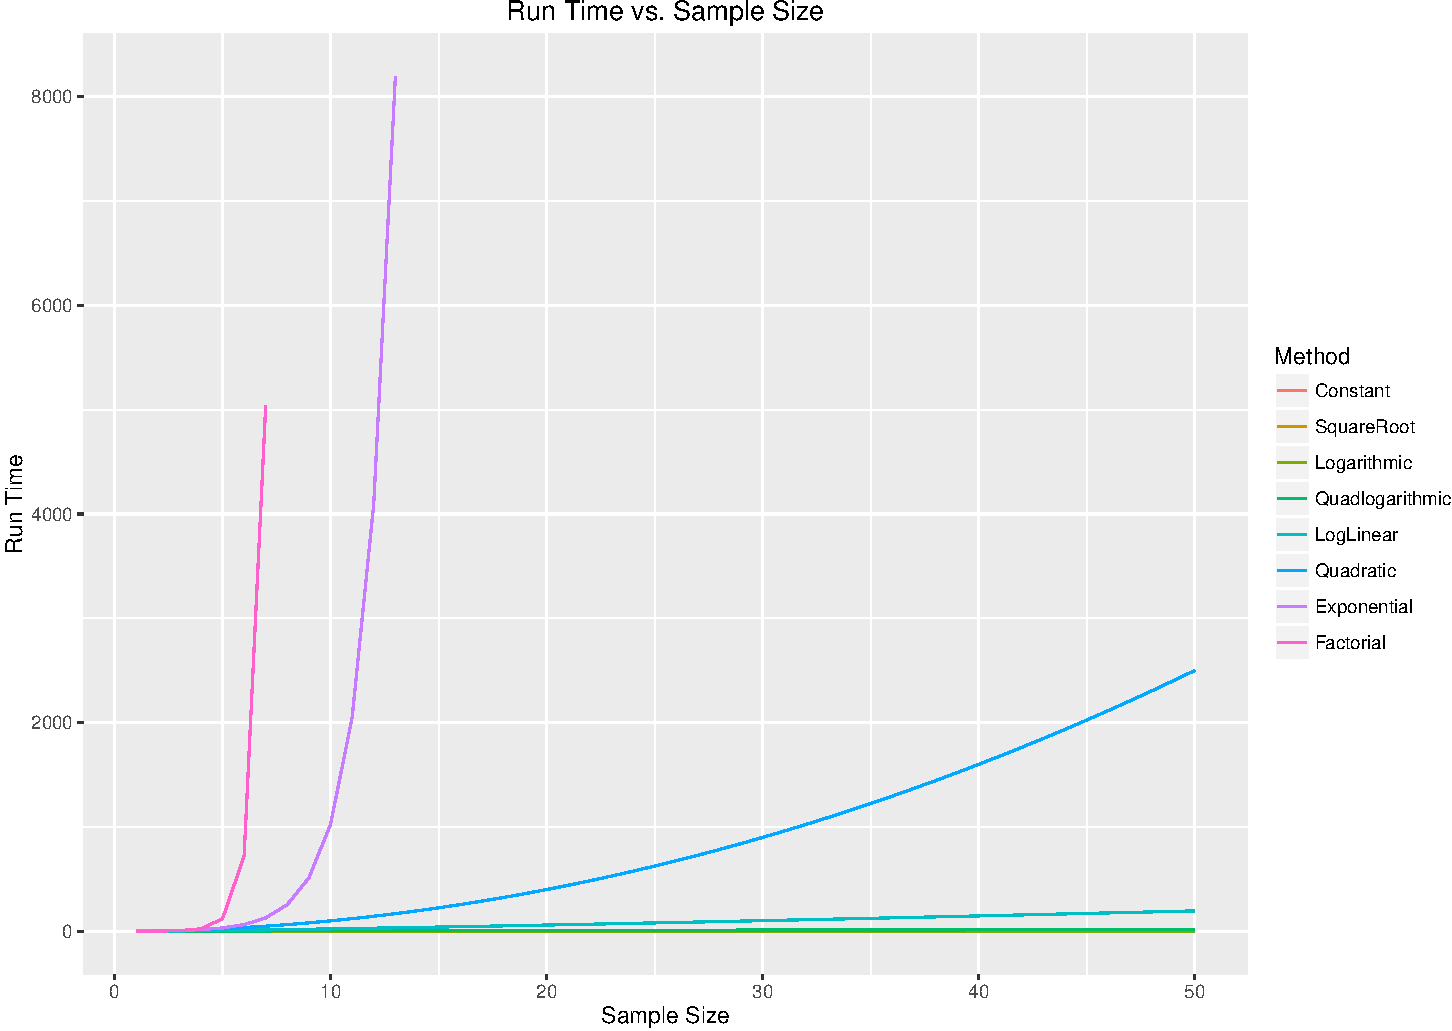
\includegraphics{lec4_grouping_big_oh_control_statements_files/figure-beamer/big_o_runtime-1.pdf}

\textbf{Note:} Even with a small sample size, certain methods take
considerably long.

\end{frame}

\begin{frame}{Few quick examples}

\begin{itemize}
\tightlist
\item
  \(O(5n) = O(n)\)
\item
  \(O(n^2 - n + 5) = O(n^2)\)
\item
  \(O(2n^3 - 8n^2 - 4n + 9) = O(n^3)\)
\item
  \(O(n^2\log(n) + n^2 + n + 1) = O(n^2\log(n))\), where \(n > 2\)
\end{itemize}

\end{frame}

\begin{frame}[fragile]{Freebies}

Within Big O, there are a few freebies that are \textbf{no cost} these
are:

\begin{itemize}
\tightlist
\item
  Function definitions
\end{itemize}

\begin{Shaded}
\begin{Highlighting}[]
\NormalTok{myfun =}\StringTok{ }\NormalTok{function(x)\{\}}
\end{Highlighting}
\end{Shaded}

\begin{itemize}
\tightlist
\item
  Return statements
\end{itemize}

\begin{Shaded}
\begin{Highlighting}[]
\KeywordTok{return}\NormalTok{(x)}
\end{Highlighting}
\end{Shaded}

\end{frame}

\begin{frame}[fragile]{Constant - Sequence of Statements}

Consider a sequence of statements:

\begin{Shaded}
\begin{Highlighting}[]
\NormalTok{statement }\DecValTok{1}
\NormalTok{statement }\DecValTok{2}
\NormalTok{...}
\NormalTok{statement n}
\end{Highlighting}
\end{Shaded}

The total time is found by adding the times for all statements:

\[T(n) = T(statement 1) + T(statement 2) + ... + T(statement n)\]

In this case, each statement is \textbf{constant} since it is
\textbf{simple} and, thus, has a Big O of: \(O(1)\).

\end{frame}

\begin{frame}[fragile]{Linear - \texttt{if/else}}

Consider an \texttt{if/else} statement

\begin{Shaded}
\begin{Highlighting}[]
\NormalTok{if (expression)\{ }\CommentTok{# True Case}
  \CommentTok{# statement 1}
\NormalTok{\} else \{         }\CommentTok{# False Case}
  \CommentTok{# statement 2}
\NormalTok{\}}
\end{Highlighting}
\end{Shaded}

Either the first statement or the second statement will run. Hence, the
worst-case or the longest run time is given by the max of:

\[\max (T(statement 1), T(statement 2))\]

\textbf{For this example,} if statement 1 is \(O(N)\) and statement 2 is
\(O(1)\) what would be the big O?

\end{frame}

\begin{frame}[fragile]{Linear - Iteration}

Consider a \texttt{for} iteration statement:

\begin{Shaded}
\begin{Highlighting}[]
\NormalTok{for(i in }\DecValTok{1}\NormalTok{:n)\{ }\CommentTok{# Loop incrementor}
  \CommentTok{# statement}
\NormalTok{\}}
\end{Highlighting}
\end{Shaded}

For this example, we assume the statement is simple, \(O(1)\).
Therefore, we are repeating this statement \(N\) times. Thus, we have
\(O(N)\).

\end{frame}

\begin{frame}{Big O Rules}

If \(T_1(n) = O(F(n))\) and \(T_2(n) = O(G(n))\), then:

\begin{itemize}
\tightlist
\item
  \(k*T_1(n) = O(F(n)))\)
\item
  \(T_1(n) + T_2(n) = \max (O(F(n)), O(G(n)))\)
\item
  \(T_1(n) * T_2(n) = O(F(n)) * O(G(n))\)
\end{itemize}

\end{frame}

\begin{frame}[fragile]{Example: Accumulative Sum on a Vector}

Often, we need to obtain summaries on vectors. Take for instance:

\begin{Shaded}
\begin{Highlighting}[]
\NormalTok{sum_vec =}\StringTok{ }\NormalTok{function(x)\{        }\CommentTok{# Cost: 0}
  \NormalTok{total_sum =}\StringTok{ }\DecValTok{0}               \CommentTok{# Cost: 1}
  
  \CommentTok{# Cost: 1 (Variable), N+1 (In Check), 2N (i = i + 1)}
  \NormalTok{for(i in }\KeywordTok{seq_len}\NormalTok{(}\KeywordTok{nrow}\NormalTok{(x)))\{}
    \CommentTok{# Cost: 2N (1 addition, 1 assignment)}
    \NormalTok{total_sum =}\StringTok{ }\NormalTok{total_sum +}\StringTok{ }\NormalTok{i }
  \NormalTok{\}}
  
  \KeywordTok{return}\NormalTok{(total_sum)           }\CommentTok{# Cost: 0}
\NormalTok{\}}
\end{Highlighting}
\end{Shaded}

The total time in this case is:

\[T(N) = 0 + 1 + 1 + (N + 1) + 2N + 2N = 5N + 2\]

which has a Big O of \(O(N)\).

\end{frame}

\begin{frame}[fragile]{Polynomial - Iteration}

Returning to iteration statements, what happens if we have three loops
inside themselves with \(K < J < I\)?

\begin{Shaded}
\begin{Highlighting}[]
\NormalTok{for(i in }\DecValTok{1}\NormalTok{:I)\{     }\CommentTok{# Loop incrementor}
  \NormalTok{for(j in }\DecValTok{1}\NormalTok{:J)\{   }\CommentTok{# Loop incrementor}
    \NormalTok{for(k in }\DecValTok{1}\NormalTok{:K)\{ }\CommentTok{# Loop incrementor}
      \CommentTok{# statement}
    \NormalTok{\}}
  \NormalTok{\}}
\NormalTok{\}}
\end{Highlighting}
\end{Shaded}

In what case could we obtain \(O(n^4)\)? How about \(O(n^{100})\)?

\end{frame}

\begin{frame}{Summary of Big O}

\begin{itemize}
\tightlist
\item
  We discussed the idea behind Big O
\item
  Observed different worst case scenarios in code
\end{itemize}

\end{frame}

\begin{frame}{References}

\hypertarget{refs}{}
\hypertarget{ref-2010tuckmangroup}{}
Tuckman, Bruce W., and Mary Ann C. Jensen. 2010. ``Stages of Small-Group
Development Revisited.'' \emph{Group Facilitation: A Research \&
Applications Journal} 10: 43--48.
\url{http://search.ebscohost.com/login.aspx?direct=true\&db=bth\&AN=49049910\&site=ehost-live}.

\end{frame}
